\documentclass[a4paper,12pt]{article}
\pdfoutput=1 % if your are submitting a pdflatex (i.e. if you have
             % images in pdf, png or jpg format)

\usepackage{jheppub} % for details on the use of the package, please
                     % see the JHEP-author-manual
\usepackage[T1]{fontenc} % if needed
\usepackage{float}
\usepackage{multicol}
\usepackage{cancel}
\usepackage[usenames,dvipsnames,svgnames,table]{xcolor}
\usepackage[a4paper,left=2.5cm,right=2.5cm,top=2.5cm,bottom=2.5cm]{geometry}
\usepackage[export]{adjustbox}
\usepackage{tikz}
\usetikzlibrary{arrows.meta}
%\graphicspath{{../calcs/}}

%\title{\boldmath A title with some math: $x=1$}
\title{CP Violation In and Beyond The Standard Model: Two Higgs Doublet Model Type II Corrections to Flavour Observables}


%% %simple case: 2 authors, same institution
%% \author{A. Uthor}
%% \author{and A. Nother Author}
%% \affiliation{Institution,\\Address, Country}

% more complex case: 4 authors, 3 institutions, 2 footn#otes
\author{Matthew Rossetter}

% The "\note" macro will give a warning: "Ignoring empty anchor..."
% you can safely ignore it.

\affiliation{Supervised By Alexander Lenz}
\affiliation{MPhys Theoretical Physics, Durham University}

% e-mail addresses: one for each author, in the same order as the authors
%\emailAdd{matthew.rossetter@durham.ac.uk}

\abstract{Abstract...}

\begin{document} 
\maketitle
%\flushbottom

\section{Introduction}
The Standard Model is one of the most successful theories ever developed, describing the fundamental forces currently observed, excluding gravity, through a quantum field theory Lagrangian, 
\begin{equation}
    \label{eq:sm}
    \begin{split}
        \mathcal{L} = -&\frac14 F^{\mu\nu}F_{\mu\nu} \qquad\qquad\qquad\quad\to \text{gauge term}\\
                      +& i\bar{\Psi}\cancel{D}\Psi \qquad\qquad\qquad\qquad\;\to \text{Fermion term} \\
                      +& (D_\mu\Phi)^\dagger(D^\mu\Phi) - V(\phi) \quad\;\;\,\to \text{Higgs term}\\
                      -& Y_{ij}\bar{\Psi}_i\Phi\Psi_j + h.c. \qquad\qquad\;\to\text{Yukawa term}
    \end{split}
\end{equation}
Throughout the latter half of the 20th century and through the 21st, the Standard Model has found strong agreement with many observed phenomena, while also predicting many other observables that took longer to be observed (most notably, the Higgs boson).
However, there are still many observations that do not align with the Standard Model; some more large scale such as unification with gravity or a description of dark matter, some more specific such as B meson oscillation frequencies or leptonic and semi-leptonic meson decays.
The modifications and additions to the Standard Model needed for these smaller scale problems could open the door to new phenomena that could bring us closer a complete theory of nature. 

\subsection{The Standard Model}
The Standard Model is a quantum field theory, describing all constituent particles as quantum fields permeating throughout space-time. 
There are twenty-five fundamental particles currently described in the Standard Model: twelve fermions (quarks and leptons), four gauge bosons of the electroweak theory ($W^\pm,Z,\gamma$), eight gluons of the strong force, and the Higgs boson.

The basis for the Standard Model are the quantum theories of electroweak and strong interactions, and then the symmetry breaking Higgs mechanism to give masses to these theories.
Both the electroweak and strong theories are non-Abelian gauge theories; the electroweak theory has a gauge symmetry of SU(2)$_{L}\otimes$U(1)$_Y$, and the strong theory of SU(3)$_{c}$ \cite{n}.
\hspace{-10pt}\footnote{The subscripts of the symmetries describe the "charge" under which particles interact with each gauge theory: $c$ represents the color charge of the strong force, $L$ states that the weak force interacts only with left-handed doublets (through which the weak isospin will be defined analagous to electric charge), and $Y$ represents the weak hypercharge of U(1) before the spontaneous symmetry breaking of the Higgs mechanism to introduce the electric charge of the electromagnetic force.\cite{o}}
\hspace{-5pt}To formulate the Standard Model Lagrangian, we start with the free Lagrangian of a massless Dirac fermion coupled to a gauge field tensor,
\begin{align}
    \label{eq:dirac:1}
    \mathcal{L} &= i\bar{\psi}\gamma^\mu\partial_\mu\psi - \frac14F^{\mu\nu}F_{\mu\nu}.
\end{align}
The Lagrangian must be formed such that it is invariant for a local gauge transformation of the fermion field, $\psi$:
\begin{equation}
    \label{eq:local}
    \psi(x)\to U(x)\psi(x),\quad \bar{\psi}(x)\to\bar{\psi}(x)U^\dagger(x),
\end{equation}
where $U(x)$ is the gauge transformation.
For U(1) and SU(N) symmetries, we have
\begin{align}
    \label{eq:gauge} 
    U_{U(1)} &= \exp\left[i\alpha\right],\quad U_{SU(N)} = \exp\left[i\alpha^a\frac{T^a}{2}\right]
\end{align}
For SU(N) symmetries, the index $a$ is summed from 1 to $N^2-1$: this is the number of gauge fields of the group.
$T^a$ are the generators of these fields, which are represented by the Pauli matrices for SU(2) and the Gell-Mann matrices for SU(3).
For SU(2), there are three gauge fields, which will lead to the three associated bosons ($W^{\pm},Z$) when mixed with U(1); and for SU(3), there are eight gauge field, leading to the eight gluons.
Clearly for U(1) there is only a single gauge field, which will lead to the photon when mixed with the SU(2) gauge fields.
In addition to the definitions in Eq.\eqref{eq:gauge}, to make Eq.\eqref{eq:dirac:1} gauge invariant, it is necessary to transform the gauge field, as well as introduce the \textit{covariant derivative}, $D_\mu$:
\begin{align}
    \label{eq:transform:1}
    A^a_\mu &\to A^a_\mu + \frac{1}{g}\partial_\mu\alpha^a + gf^{abc}\alpha^bA^c_\mu, \\
    \label{eq:transform:2}
    \partial_\mu &\to D_\mu = \partial_\mu - igT^aA^a_\mu,
\end{align}
where $g$ is the relevant gauge coupling parameter.
The full covariant derivative of the Standard Model is
\begin{equation}
    \label{eq:covar}
    D_\mu = \partial_\mu - ig_1\frac{Y}{2}B_\mu - ig_2\frac{\sigma^i}{2}W^i_\mu - ig_3\frac{\lambda^a}{2}G^a_\mu,
\end{equation}
combining all constituent gauge groups, with $g_{1,2,3}$ the gauge coupling of U(1)$_Y$, SU(2)$_L$, and SU(3)$_c$ respectively where the gauge field(s) and generator(s) of each group are in the term of their coupling \cite{m}.   
Note that Eqs.\eqref{eq:transform:1} and \eqref{eq:transform:2} are the general forms for the SU(N) theories; if considering U(1), these are simplified.
From these definitions, the gauge invariance of Eq.\eqref{eq:dirac:1} for U(1) symmetry is trivial, and for SU(N) symmetries, it will simply follow after defining a commutation relation between generators:
\begin{equation}
    \label{eq:commute}
    [T^a,T^b] = if^{abc}T^c,
\end{equation}
where $f^{abc}$ are the structure constants which define each SU(N) group \cite{n}. 
It can be useful to define the fermion spinor $\psi$ into an upper and lower part, which can be done in many ways, but it is important in the formulation of the Standard Model to separate the fermion field into left- and right-handed components. 
To this end, we define the operators
\begin{align}
    \label{eq:helix}
    P_L &= \frac{1-\gamma^5}{2}, & P_R &= \frac{1+\gamma^5}{2},
\end{align}
where $\gamma^5$ is defined in the conventional representation. 
The left-handed projection of the fermion field $\psi$ would then be
\begin{equation}
    \label{eq:projection}
    \psi_L = P_L\psi.
\end{equation}
Now when forming the SU(2) symmetry of the weak force, there is a difference between the interaction of right- and left-handed fermions; that is, left-handed fermions transform under the SU(2) space, whereas right-handed do not.
Considering both quarks and leptons in the traditional three generations, then under the electroweak SU(2) space, each generation forms a left-handed doublet and a right-handed singlet, e.g.
\begin{align}
    \label{eq:doublet}
    \Psi_L &=\begin{pmatrix} \nu_e \\ e^- \end{pmatrix}_L,\; e_R^-, & \Psi_{L\alpha} &=\begin{pmatrix} u_\alpha \\ d_\alpha\end{pmatrix}_L,\; u_{R\alpha},d_{R\alpha},
\end{align}
where $\alpha$ represents the colour charge of the quarks under the strong interaction \cite{m}.
Neutrinos only appear in the left-handed doublets and do not form right-handed singlets, as there is currently no experimental evidence for their existence.
So right- and left-handed fermions are in different SU(2) multiplets; this represents a parity violation in the Standard Model which is also found in nature. 
This is an important criterion of a theory of nature, as will be discussed more in section \ref{subsec:flavobs}.

Gauge symmetry has thus far yielded a Lagrangian to describe fermions and forces and their interactions, but only for massless particles, but this is not observed in nature. 
For massive fermions and bosons respectively, the Lagrangian would require terms of the form $m\bar{\psi}\psi$ and $m_A^2A_\mu A^\mu$.
The fermion mass term would initially seem invariant, but under the electroweak symmetry, it is rewritten as
\begin{equation}
    \label{eq:mass}
    m\bar{\psi}\psi = m(\bar{\psi}_R\psi_L+\bar{\psi}_L\psi_R),
\end{equation}
and so is no longer invariant, due to the mixing of right-handed and left-handed spinors. 

To solve this problem, the Higgs mechanism can be introduced as a way to spontaneously break the symmetry of the electroweak force to generate massive bosons. 
The Lagrangian of the scalar Higgs reads
\begin{equation}
    \label{eq:higgslag}
    \mathcal{L} = (D^\mu\phi)^\dagger(D_\mu\phi) - V(\phi).
\end{equation}
Consider a complex scalar field under the SU(2) left-handed doublet representation,
\begin{equation}
    \label{eq:doubscal}
    \Phi = \frac{1}{\sqrt{2}}\begin{pmatrix}\phi_1+i\phi_2\\\phi_0+i\phi_3\end{pmatrix} = \begin{pmatrix} \phi^+\\\phi^0\end{pmatrix},
\end{equation}
which has a U(1) hypercharge $Y=+\frac12$ \cite{l}.
The covariant derivative in Eq.\eqref{eq:higgslag} is that defined for SU(2)$\otimes$U(1):
\begin{equation}
    \label{eq:covarhiggs}
    D_\mu\phi = \left(\partial_\mu + igT^iW_\mu^i + \frac{i}{2}g'B_\mu\right)\phi,
\end{equation}
with $W^i_\mu$ and $B_\mu$ the gauge fields of SU(2)$_L$ and U(1)$_Y$, and $g$ and $g'$ the SU(2) and U(1) gauge couplings respectively. 
The Higgs potential $V(\phi)$ in Eq.\eqref{eq:higgslag} is defined as
\begin{equation}
    \label{eq:goldpot}
    V(\phi) = -\mu^2\phi^\dagger\phi + \lambda(\phi^\dagger\phi)^2.
\end{equation}
If $\mu^2>0$, then the scalar field will acquire a non-zero vacuum expectation value (VEV), which will spontaneously break the symmetry. 
The VEV can be defined as
\begin{equation}
    \label{eq:vev}
    \langle\phi\rangle = \frac{1}{\sqrt{2}}\begin{pmatrix}0\\v\end{pmatrix}.
\end{equation}
To ensure that the symmetry of electromagnetism is not broken, the scalar field $\phi^0$ is taken to have charge $Q=0$.
Under this scheme, both the hypercharge $Y$ and the weak isospin $T_3$ are not conserved, but the specific combination of them which is defined as electric charge, $Q=T_3+\frac12 Y$ is conserved, so the electroweak symmetry is spontaneously broken to form a U(1) symmetry of electric charge $Q$,
\begin{equation}
    \label{eq:symbreak}
    SU(2)_L\otimes U(1)_Y \to U(1)_Q.
\end{equation}
The $W^\pm$ and $Z$ masses can now be generated from this mechanism. 
In the unitary gauge, the scalar doublet can be written
\begin{equation}
    \label{eq:unig}
    \Phi = \frac{1}{\sqrt{2}}\begin{pmatrix}0\\v+h\end{pmatrix}.
\end{equation}
Through substituting the above into Eq.\eqref{eq:higgslag}, the gauge fields of the real electroweak bosons $W^{\pm},Z,\gamma$ can be found as linear combinations of $W^i_\mu$ and $B_\mu$ with their mass terms now generated in a gauge invariant form:
\begin{align}
    \label{eq:gagmix}
    W^\pm_\mu &\equiv \frac{1}{\sqrt{2}}(W_\mu^1 \mp iW_\mu^2), & m_W &= \frac{gv}{2}, \\
    Z_\mu &\equiv \frac{1}{\sqrt{g^2+g'^2}}(gW^3_\mu-g'B_\mu), & m_Z &= \frac{v}{2}\sqrt{g^2+g'^2}\\
    A_\mu &\equiv \frac{1}{\sqrt{g^2+g'^2}}(g'W_\mu^3+gB_\mu), & m_A &= 0.
\end{align}
It can be said that three of component scalar fields in Eq.\eqref{eq:doubscal} were "eaten" to form the gauge boson masses, and the fourth field goes on to become the Higgs phenomenon \cite{o}.\\
Now the final piece of the puzzle is fermion masses. 
We consider the final term of Eq.\eqref{eq:sm}, the Yukawa Lagrangian. 
It is split into terms, the one written and "h.c.", representing the hermitian conjugate of the former.
The hermitian conjugate term is required so both up-type quarks, and down-type quarks and charged leptons gain mass \cite{m}. 
In the unitary gauge, the down-type quark Yukawa term reads
\begin{align}
    \label{eq:yuk}
    -\mathcal{L}_{Yuk}^d = \sum_{a,b} Y^{(d)}_{ab} \begin{pmatrix} \bar{u}_{aL} & \bar{d}_{aL}\end{pmatrix}\begin{pmatrix}0\\\frac{v}{\sqrt{2}}\end{pmatrix}d_{bR} = \sum_{a,b}Y^{(d)}_{ab}\phi_0\bar{d}_{aL}d_{bR},
\end{align}
where $\phi^0$ is defined as $\frac{v}{\sqrt{2}}$ through the transformation
\begin{align}
    \label{eq:vtoh}
    \Phi = \frac{1}{\sqrt{2}}\begin{pmatrix}0\\v+h\end{pmatrix}\to\frac{1}{\sqrt{2}}\begin{pmatrix}0\\v\end{pmatrix}
\end{align}
from the spontaneous symmetry breaking. 
So now down-type quarks and charged leptons have gained masses. 
To generate the masses of the up-type quarks and charged leptons, the hermitian cojugate term is used, where now a second Higgs doublet (not dependent of the first, but its charge-conjugate) is introduced as
\begin{align}
    \label{eq:highc}
    \tilde{\Phi} &= i\sigma_2\Phi^* = \begin{pmatrix}\phi^{0*}\\-\phi^{+*}\end{pmatrix} = \frac{1}{\sqrt{2}}\begin{pmatrix}v+h\\0\end{pmatrix}.
\end{align}
The up-type quark Yukawa term is then
\begin{align}
    \label{eq:yukhc}
    -\mathcal{L}_{Yuk}^u = \sum_{a,b} Y^{(u)}_{ab}\begin{pmatrix}\bar{u}_{aL} & \bar{d}_{aL}\end{pmatrix}\begin{pmatrix}\frac{v}{\sqrt{2}}\\0\end{pmatrix}u_{bR} = \sum_{a,b}Y^{(u)}_{ab}\phi^0\bar{u}_{aL}u_{bR}.
\end{align}
The charged lepton masses are generated similarly, and the expressions of masses read
\begin{align}
    \label{eq:fermas}
    m_i = -\frac{Y_iv}{\sqrt{2}},
\end{align}
where $i$ represents whichever fermion is in question \cite{o}. 
The question of neutrino mass is at the forefront of some research, and so won't be mentioned in this study, other than that it is now known that neutrinos do have mass, however small. 

In Eqs.\eqref{eq:yuk} and \eqref{eq:yukhc}, we have formed non-diagonal mass matrices. 
These can be diagonalised in which the constituent states are the mass eigenstates, e.g. for the quarks, there would be 
\begin{align}
    \label{eq:massmat}
    \frac{v}{\sqrt{2}}V_1^\dagger Y_uV_1 &= \begin{pmatrix} m_u & & \\ & m_c & \\ & & m_t\end{pmatrix}, & \frac{v}{\sqrt{2}}V_2^\dagger Y_dV_2 &= \begin{pmatrix} m_d & & \\ & m_s & \\ & & m_b\end{pmatrix}.
\end{align}
However these cannot both be diagonalised simultaneously. 
By convention, it is chosen to diagonalise the up-type quarks, and then rotate the down-type quarks between their weak eigenstates and their mass eigenstates \cite{l}. 
The famous CKM matrix, defined $V_{CKM}\equiv V_1^\dagger V_2$, is the matrix connecting to mass and weak eigenstates,
\begin{equation}
    \label{eq:ckmone}
    \begin{pmatrix} d \\ s \\ b\end{pmatrix} = V_{CKM}\begin{pmatrix} d' \\ s' \\ b'\end{pmatrix},
\end{equation}
as well as describing quark mixing between the up- and down-type quarks. 
The CKM matrix in its full form is a unitary matrix; it is currently believed to be a $3\times3$ unitary matrix, however this could be section of a $4\times4$ unitary matrix if a fourth generation of fermions existed, meaning the current $3\times3$ matrix would not be unitary. 
The strengths of quark coupling are stored in elements of the CKM matrix as
\begin{align}
    \label{eq:ckmub}
    V_{CKM} &= \begin{pmatrix}V_{ud}&V_{us}&V_{ub}\\V_{cd}&V_{cs}&V_{cb}\\V_{td}&V_{ts}&V_{tb}\end{pmatrix}.
\end{align}
These individual elements can be found through quark coupling processes. 
For better understanding of the CKM matrix however, it can be easier to parameterise it. 
There are many parameterisations that can be used for this, though the two most common are the \emph{standard parameterisation} and the \emph{Wolfenstein parameterisation} \cite{l}.
The standard parameterisation follows from extension of the Cabibbo angle for first and second generation mixing, where we now use three Cabibbo-like matrices for interactions of two quark generations, and multiply them for the CKM matrix, including a phase required by the formation of a $3\times3$ unitary matrix:
\begin{equation}
    \label{eq:standpar}
    \begin{split}
        V_{CKM} &= \begin{pmatrix}1&0&0\\0&\cos\theta_{23}&\sin\theta_{23}\\0&-\sin\theta_{23}&\cos\theta_{23}\end{pmatrix}\begin{pmatrix}\cos\theta_{13}&0&\sin\theta_{13}e^{i\delta}\\0&1&0\\-\sin\theta_{13}e^{i\delta}&0&\cos\theta_{13}\end{pmatrix}\begin{pmatrix}\cos\theta_{12}&\sin\theta_{12}&0\\-\sin\theta_{12}&\cos\theta_{12}&0\\0&0&1\end{pmatrix}\\
                &= \begin{pmatrix}c_{12}c_{13} & s_{12}c_{13} & s_{13}e^{-i\delta} \\ -s_{12}c_{23}-c_{12}s_{23}s_{13}e^{i\delta} & c_{12}c_{23}-s_{12}s_{23}s_{13}e^{i\delta} & s_{23}c_{13} \\ s_{12}c_{23}-c_{12}c_{23}s_{13}e^{i\delta} & -c_{12}s_{23}-s_{12}c_{23}s_{12}e^{i\delta} & c_{23}c_{13}\end{pmatrix}
    \end{split}
\end{equation}
The Wolfenstein parameterisation approximates the standard parameterisation as $\lambda=s_{12}\approx0.22543$, $A\lambda^2=s_{23}$, and $A\lambda^3(\rho-i\eta)=s_{13}e^{-i\delta}$, and performs a Taylor expansion traditionally to order $\lambda^3$ to yield
\begin{align}
    \label{eq:wolfie}
    V_{CKM} &= \begin{pmatrix} 1-\frac{\lambda^2}{2} & \lambda & A\lambda^3(\rho-i\eta) \\ -\lambda & 1-\frac{\lambda^2}{2} & A\lambda^2 \\ A\lambda^3(1-\rho-i\eta) & -A\lambda^2 & 1\end{pmatrix} + \mathcal{O}(\lambda^4).
\end{align}
This parameterisation makes it very easy to see the relative strengths of the coupling. 

An important element of the CKM matrix is its complex phase.
\hspace{-10pt}\footnote{If its real form were a $4\times4$ matrix, there would be three phases.}
\hspace{-5pt}The presence of a complex phase allows for CP-violating processes to take place in the Standard Model: the CKM matrix's Hermitian conjugate will give the complex conjugated phase, yielding different physics over CP conjugation for complex coupling elements. 
In the Wolfenstein parameterisation, all CP violation is held with the $\rho-i\eta$ terms. 
Plotting measurements in the $(\rho,\eta)$ plane can prove useful in understanding these terms, to which end, the unitarity triangle can be formed:
\begin{figure}[H]
    \centering
    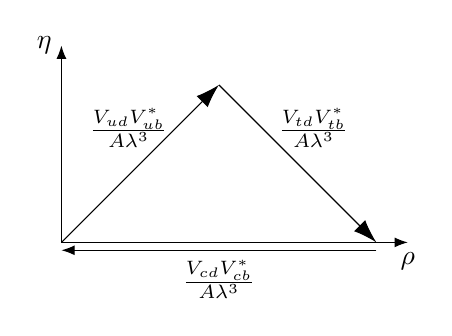
\begin{tikzpicture}
        \draw[-Latex] (0,0) -- (4.4,0) node[anchor=north] {$\rho$};
        \draw[-Latex] (0,0) -- (0,2.5) node[anchor=east] {$\eta$};
        \draw[-{Latex[length=3mm,width=2mm]}] (0,0) -- (2,2) node[anchor=north east,xshift=-15pt,yshift=-5pt] {$\frac{V_{ud}V_{ub}^*}{A\lambda^3}$};
        \draw[-{Latex[length=3mm,width=2mm]}] (2,2) node[anchor=north west,xshift=18pt,yshift=-5pt] {$\frac{V_{td}V_{tb}^*}{A\lambda^3}$} -- (4,0);
        \draw[-Latex] (4,-0.1) -- (0,-0.1) node[anchor=north,midway] {$\frac{V_{cd}V_{cb}^*}{A\lambda^3}$};
    \end{tikzpicture}
    \caption{\label{fig:unitang} The unitarity triangle from the Wolfenstein parameterisation in $(\rho,\eta)$ space.}
\end{figure}
The unitarity triangle can help describe many things in quark mixing, such as Cp violation, through the length of its side and its angles. 
It can also be useful to define a unitarity circle through comparison of experiment and theory in CP violating processes, and from these and others, many regions in the $(\rho,\eta)$ plane can be defined to interpret various constants and effects in quark mixing. 
\begin{figure}[H]
    \centering
    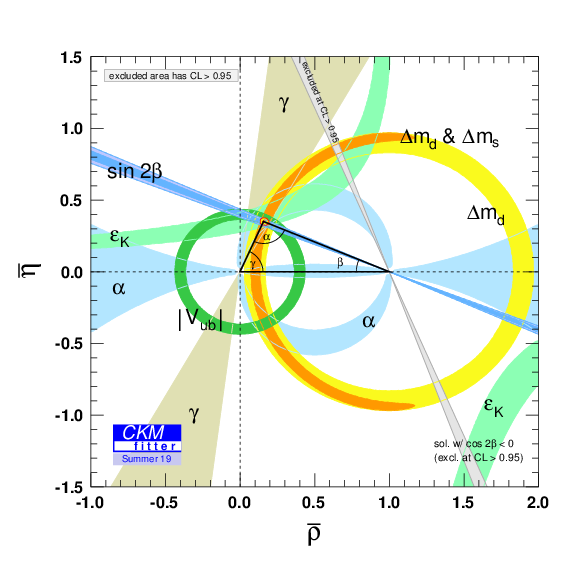
\includegraphics[scale=0.5]{rhoeta_large.png}
    \caption{\label{fig:ckmfitter} The global CKM fit in the $(\rho,\eta)$ plane, as of 13/01/20 \cite{g}.}
\end{figure}

\subsection{Flavour Physics and CP Violation}
\label{subsec:flavobs}
A significant focus of flavour physics is the study of CP violation - the violation of CP symmetry (the product of Charge and Parity symmetries) in the Standard Model.
CP symmetry was introduced as a candidate for the fundamental symmetry of Standard Model interactions after Parity violation was discovered in the 1950s.
One of the big questions about the formulation of our universe is why is there an asymmetry between matter and anti-matter. 
One of the conditions Sakharov found in 1967 to answer this question is a necessity of CP violation \cite{h}; if left-handed baryons interact differently to right-handed anti-baryons, then one of these can be more prominent than the other. 
Both the electromagnetic and strong forces appear to conserve CP, however the weak force, through the chiral nature of its couplings, does not.
Through the weak force, there are two ways for CP violating interactions to occur: through complex Yukawa couplings in the CKM matrix; through complex Higgs parameters, such as those in the 2 Higgs Doublet Model to be discussed in section \ref{subsec:2hdm}.
There is also a question of whether CP violation can be found in the strong sector, but this will not be discussed here \cite{m}.

Currently, there are two cruxes to the study of Sakharov's condition of CP violation: experiment finds larger scattering amplitudes than theory for many CP-violating processes; and the amount of CP violation currently observed would not be enough to account for the large baryon asymmetry of the universe. 
Both these cruxes point towards physics beyond the Standard Model to add to the CP violation predicted and perhaps predict where to observe the CP violation needed in nature \cite{l}. 
There are many proposals for Standard Model extensions which could bridge the gap between theory and experiment, although these extensions would require new particles to be observed to explain their phenomena, none of which have so far been observed. 

The $Z'$ boson is a common extension to the Standard Model, which in its simplest application behaves akin to the $Z^0$ boson but with a higher mass. 
There are many descriptions of the $Z'$ boson ranging from the introduction of a new U(1) gauge symmetry to the inclusion of string theory. 
The consideration of a $Z'$ boson to flavour physics is to add extra coupling paths to scattering amplitudes which could better explain flavour observables. 
An example of how $Z'$ could modify Standard Model decays is given in Figure \ref{fig:bmes}.
\begin{figure}[H]
    \vspace{-20pt}
    \begin{equation}
        \Gamma_{\text{Exp}} = 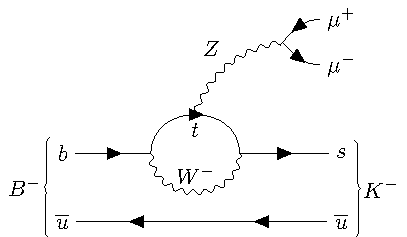
\includegraphics[scale=0.8,raise=-16pt]{../notes/bminus.pdf} + 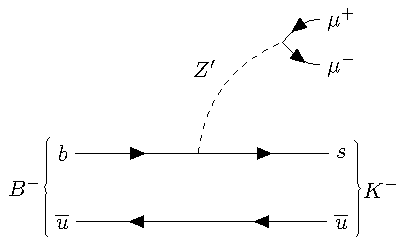
\includegraphics[scale=0.8,raise=-16pt]{../notes/bminusprime.pdf}
    \end{equation}
    \caption{\label{fig:bmes} Proposed $Z'$ model extension to $\Gamma[B^-\to K^-\mu^+\mu^-]_{SM}$}
\end{figure}

It could also be possible that there is a fourth generation of fermions, perfectly replicating the first generation to higher masses as the second and third generations do. 
The presence of the fourth generation could add extra Feynman diagrams to decays, increasing the resulting decay amplitude. 
Another interesting implication of a fourth generation would be that the CKM matrix would now be a 4x4 matrix, which could see some alterations to flavour-changing interactions, perhaps even some additional complex terms where CP violation would arise. 
A key indicator on this extension is in the Higgs mechanism. 
\begin{figure}[H]
    \centering
    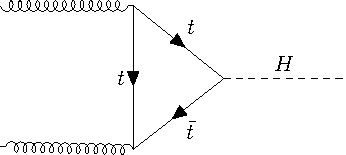
\includegraphics{../notes/higgs.pdf}
    \caption{\label{fig:higgs} Higgs boson production through the top quark loop.}
\end{figure}
The Higgs couples more strongly to heavier particles, so the top-Higgs interaction seen in \ref{fig:higgs} should be replicated with the theoretical $t'$ and $b'$ quarks with increased amplitudes. 
However, when just considering the SM4 model, the new prediction of the Higgs scattering amplitude is far greater than that observed. 
It could be possible that the SM4 model is physical, but would also need another extension to resolve its issues, such as the Two Higgs Doublet Model discussed below. 

Whenever constructing new theories to extend the Standard Model, the inspiration can frequently come from a few specific cases of inconsistency. 
However it is important to test these extensions across all observables which could involve the new processes.
If the extension resolves issues with some observables while creating new ones with others, then it is of no use; only extensions which work across the whole spectrum of phenomena can be physical. 

\subsection{The Two Higgs Doublet Model of Type II}
\label{subsec:2hdm}
Previously in the Standard Model Higgs mechanism, to generate the masses of the weak gauge bosons and fermions, a single Higgs SU(2) doublet of complex scalar fields was introduced, as in Eq.\eqref{eq:doubscal}.
To form masses for both up- and down-type quarks and charged leptons, we introduced the hermitian conjugate doublet in Eq.\eqref{eq:highc}, otherwise the Higgs field would only give mass to the down-type quarks. 
Instead, two Higgs doublets can be postulated, of the general form
\begin{align}
    \label{eq:gdbl}
    \Phi_1 &= \begin{pmatrix} \phi_1 + i\phi_2 \\ \phi_0 + i\phi_3\end{pmatrix}, & \Phi_2 &= \begin{pmatrix} \phi_5+i\phi_6\\\phi_4+i\phi_7\end{pmatrix}.
\end{align}
These two doublets would have opposite hypercharge so one would couple to up-type quarks, and the other to down-type, thus requiring no need for a conjugate field. 
Each doublet would have its own VEV, with the quadrature addition of these two VEVs creating the value known in the Standard Model:
\begin{align}
    \label{eq:dbldbl}
    \Phi_1 &= \frac{1}{\sqrt{2}}\begin{pmatrix}0\\v_1\end{pmatrix}, & \Phi_2 &= \frac{1}{\sqrt{2}}\begin{pmatrix}v_2\\0\end{pmatrix}, & v_{SM}^2 &= v_1^2 + v_2^2.
\end{align}
Under this model, the masses of the three weak gauge bosons can still be generated in the same way, each eating one of the scalar fields, however this time there would be 5 residual scalar fields, and so, five Higgs fields should be found: three neutral Higgs, two scalar $H$ and $h$ (where $h$ is the SM Higgs particle) and one pseudoscalar $A$; and two charged Higgs $H^\pm$.
The introduction of these new particles requires searching for additional parameters to describe them: the masses of $H$, $A$, and $H^\pm$; the mixing angle between $h$ and $H$; and the VEV ratio $\tan\beta=v_2/v_1$.

The two Higgs doublet model (2HDM) described above is the type II version, where $\Phi_1$ couples to down-type quarks and $\Phi_2$ couples to up-type quarks and charged leptons. 
There are other types of 2HDM where the two Higgs doublets couple in different ways, but the promising sign from Type II is that it yields a similar expression for the Yukawa Lagrangian to the SM. 
This in turn yields a similar CKM matrix through which all flavour-changing interactions can be described. 
The addition of 4 new Higgs fields introduces new interactions, where the charged Higgs fields can replace $W$ fields in flavour-changing charged interactions, as well as additional neutral interactions between the neutral Higgs scalar and pseudoscalar fields. 

The presence of charged Higgs fields presents the opportunity to bridge the gap between theory and experiment. 
The charged Higgs particles can mediate weak charged currents in the same way as $W^{\pm}$, and the additional contribution of $H^{\pm}$ to many weak-mediated decays could correct the Standard Model to correctly predict these decay paths. 
The important factors to determine whether these charged Higgs could be the answer to the inconsistencies are the relevant parameters from the 2HDM: the charged Higgs mass $m_{H^+}$, and the VEV ratio $\tan\beta$. 
Values of these parameters which align theory and observation can indicate where LHC experiments can probe for these theorised new particles. 
If either these particles cannot be found, or are found with parameters that do not lie in regions of agreement, then there must be some other factors at play yet to be addressed. 
This study considers where regions of the 2HDM Type II parameters can align SM predictions with experiment, giving indication of where they could be found in nature if this model is to be a real extension of the Standard Model.

\section{Probing the 2HDM Type II}
\label{sec:probe}
Below will follow \cite{a} closely in describing the SM theory for the decays relevant to charged Higgs searches and extending these into the 2HDM. 
The measurements and parameters used for these expressions is given in \emph{table}.

\subsection{Leptonic Decays}
\label{subsec:lep}
In the Standard Model, the leptonic decay $M\to l\nu_l$, where $M$ is a charged meson, has a branching ratio of
\begin{equation}
    \label{eq:mlv}
    \mathcal{B}[M\to l\nu_l]_{\text{SM}} = \frac{G_F^2m_Mm_l^2}{8\pi}\left(1-\frac{m_l^2}{m_M^2}\right)^2 |V_{q_uq_d}|^2f_M^2\tau_M(1+\delta_{EM}^{Ml2}),
\end{equation}
where $q_u$ and $q_d$ represent the up- and down-like quarks of the meson, $V_{q_uq_d}$ the CKM element, and $f_M$ the $M$ meson's decay constant.
$\delta_{EM}^{Ml2}$ is a corrective factor for electromagnetic radiative corrections. 
For $\pi$ and $K$ mesons, the effect is around 2-3\%, and around 1\% for $D$ mesons.
For $B$ meson phenomena, the effect is approximated to 0. 

For the light mesons, kaons and pions, it is easier to determine the ratio of their decay constants $f_K/f_\pi$ than the individual values, and so it is then easier to consider the ratio of their branching fractions as well. 
In the Standard Model, 
\begin{equation}
    \label{eq:kpi}
    \frac{\Gamma[K\to\mu\nu]_{\text{SM}}}{\Gamma[\pi\to\mu\nu]_{\text{SM}}} = \frac{m_K}{m_\pi}\left(\frac{1-m_l^2/m_K^2}{1-m_l^2/m_\pi^2}\right)^2 \bigg|\frac{V_{us}}{V_{ud}}\bigg|^2\left(\frac{f_K}{f_\pi}\right)^2(1+\delta^{Kl2/\pi l2}_{EM}).
\end{equation}
It is also worth considering the ratio of tau decays of kaons to pions:
\begin{equation}
    \label{ep:tkpi}
    \frac{\Gamma[\tau\to K\nu]_{\text{SM}}}{\Gamma[\tau\to\pi\nu]_{\text{SM}}} = \left(\frac{1-m_K^2/m_\tau^2}{1-m_\pi^2/m_\tau^2}\right)^2\bigg|\frac{V_{us}}{V_{ud}}\bigg|^2\left(\frac{f_K}{f_\pi}\right)^2(1+\delta_{EM}^{\tau K2/\tau\pi2}).
\end{equation}

These SM branching values will take alterations from the two Higgs doublet model of the form
\begin{equation}
    \label{eq:mesrh}
    \mathcal{B}[M\to l\nu] = \mathcal{B}[M\to l\nu]_{\text{SM}}(1+r_H)^2,
\end{equation}
where $r_H$ is the corrective factor of the two Higgs doublet model:
\begin{align}
    \label{eq:rh}
    r_H &= \left(\frac{m_{q_u}-m_{q_d}\tan^2\beta}{m_{q_u}+m_{q_d}}\right)\left(\frac{m_M}{m_{H^+}}\right)^2.
\end{align}
It can still be possible through this method for some leptonic decays to have agreement between the SM predictions and experiment, where $r_H = 0,-2$.
$r_H=0$ is known as the decoupling solution which can be found as $m_{H^+}$ approaches infinity; $r_H=-2$, the fine-tuned solution, is obtained from a linear relationship between $m_{H^+}$ and $\tan\beta$, which will be dependent of the masses of the meson and its constituent quarks, so will vary between mesons. 


\subsection{Mass mixing}
\label{subsec:mix}
Neutral B meson mixing is a common study in flavour physics, due to the strong dependence on the heavy $W$ exchange. 
\begin{figure}[H]
    \centering
    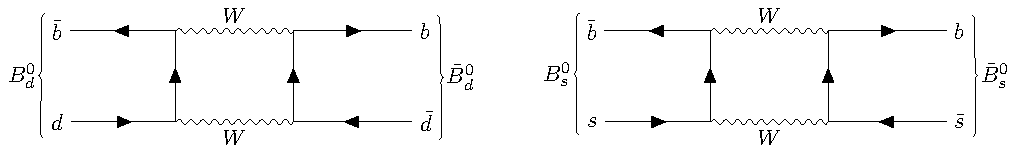
\includegraphics[width=\textwidth]{bmix.pdf}
    \caption{\label{fig:bmix} Box diagrams detailing $B_d$ and $B_s$ meson mixing.}
\end{figure}
In 2HDM, the mass difference between the two mixed states receives two additional contributions from box diagrams using the heavy charged Higgs in place of both $W$s or one $W$. 
For $B_q$, where $q=d,s$, this results in:
\begin{align}
    \Delta m_q &= \frac{G_F^2}{24\pi^2}(V_{tq}V_{tb}^*)^2\eta_Bm_Bm_t^2f_{B_q}^2\hat{B}_{B_q}(S_{WW}+S_{WH}+S_{HH}), \\
    S_{WW} &= \left(1+\frac{9}{1-x_{tW}}-\frac{6}{(1-x_{tW})^2}-\frac{6x_{tW}^2\ln(x_{tW})}{(1-x_{tW})^3}\right), \\
    S_{WH} &= \frac{x_{tH}}{\tan^2\beta}\left(\frac{(2x_{HW}-8)\ln(x_{tH})}{(1-x_{HW})(1-x_{tH})^2}+\frac{6x_{HW}\ln(x_{tW})}{(1-x_{tW})(1-x_{tW})^2}-\frac{8-2x_{tW}}{(1-x_{tW})(1-x_{tH})}\right),\\
    S_{HH} &= \frac{x_{tH}}{\tan^4\beta}\left(\frac{1+x_{tH}}{(1-x_{tH})^2}+\frac{2x_{tH}\ln(x_{tH})}{(1-x_{tH})^3}\right),
\end{align}
where $x_{ij} = m_i^2/m_j^2$, and $S_{xy}$ describes the internal bosonic lines for the two bosons $x,y = H^\pm,W^\pm$.
The current SM calculations for the mass differences are calculated in \cite{i} to be
\begin{align}
    \Delta m^{\text{SM}}_d &= \left(0.533^{+0.022}_{-0.036}\right)ps^{-1} = \left(1.05^{+0.04}_{-0.07}\right)\Delta m_d^{\text{exp}}, \\
    \Delta m^{\text{SM}}_s &= \left(18.4^{+0.7}_{-1.2}\right)ps^{-1} = \left(1.04^{+0.04}_{-0.07}\right)\Delta m_s^{\text{exp}}.
\end{align}

\subsection{Radiative decay}
\label{subsec:rad}
The radiative decay $b\to s\gamma$ occurs through the flavour-changing neutral currents of penguin diagrams.
The Standard Model calculations of $\bar{B}\to X_s\gamma$ have been performed up to Next-to-Next Leading Order (NNLO), which yields a complicated expression, so the result is parameterised in line with \cite{a,b}.
\begin{figure}[H]
    \centering
    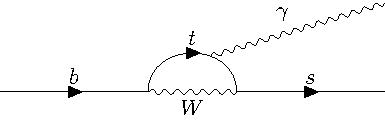
\includegraphics[scale=1.2]{bsgam.pdf}
    \caption{\label{fig:bsgam} A one-loop penguin diagram for $b\to s\gamma$ decay.}
\end{figure}
Similarly to B meson mixing, W can be substituted for a charged Higgs in all the relevant penguin diagrams, giving extra contributions again to the theory. 
The 2HDM corrections given by these additional contributions are calculated to NLO in \cite{b}, so the SM parameters must be limited to NLO.
The normalised branching ratio of $\bar{B}\to X_s\gamma$ is given by
\begin{equation}
    \label{eq:xsgam}
    \mathcal{R}_{b\to s\gamma} = \frac{\mathcal{B}[\bar{B}\to X_s\gamma]}{\mathcal{B}[\bar{B}\to X_cl\bar{\nu}]} = \bigg|\frac{V_{ts}^*V_{tb}}{V_{cb}}\bigg|^2 \frac{6\alpha_{\text{EM}}}{\pi C}(P+N).
\end{equation}
Here, $P$ represents the perturbative leading contribution in the heavy quark expansion, and $N$ the non-perturbative higher-order contributions of the heavy quark expansion.
$P$ and $N$ are parameterised in \cite{a,b} as 
\begin{equation}
    \label{eq:pplsn}
    P+N = (C^{\text{eff},(0)}_{7,SM}+B\Delta C_{7,H^+}^{\text{eff},(0)})^2+A,
\end{equation}
where $A$ and $B$ are functions defined in \cite{a}, $C_{7,SM}^{\text{eff},(0)}$ is one of the Wilson coefficients of the effective Hamiltonian in the SM, and $\Delta C_{7,H^+}^{\text{eff},(0)}$ holds the charged Higgs contributions to the SM Wilson coefficient. 

In Eq.\eqref{eq:xsgam}, $C$ is a phase space normalisation factor for the difference between the two branching ratios. 
From \cite{f}, it is defined as 
\begin{align}
    \label{eq:phasespace}
    C &= \bigg|\frac{V_{ub}}{V_{cb}}\bigg|^2\frac{\Gamma(\bar{B}\to X_ce\bar{\nu})}{\Gamma(\bar{B}\to X_ue\bar{\nu})}.
\end{align}

\subsection{Input and Fits}
\label{subsec:fit}
\begin{table}[H]
    \centering
    \begin{tabular}{c|ccc}
        \hline\hline
        Branching Ratios & Value & Unit & Reference \\
        \hline\hline
        $\mathcal{B}[B\to\tau\nu]$ & $1.09\pm0.24$ & $10^{-4}$ & \cite{d} \\
        $\mathcal{B}[D\to\mu\nu]$ & $3.82\pm0.33$ & $10^{-4}$ & \cite{d} \\
        $\mathcal{B}[D_s\to\tau\nu]$ & $5.48\pm0.23$ & $10^{-2}$ & \cite{d} \\
        $\Gamma[K\to\mu\nu]/\Gamma[\pi\to\mu\nu]$ & $1.337\pm0.003$ & & \cite{d} \\
        $\Gamma[\tau\to K\nu]/\Gamma[\tau\to\pi\nu]$ & $6.438\pm0.094$ & $10^{-2}$ & \cite{d} \\
        $\Delta m_d$ & $0.5064\pm0.0019$ & $ps^{-1}$ & \cite{c} \\ 
        $\Delta m_s$ & $17.757\pm0.021$ & $ps^{-1}$ & \cite{c} \\
        $\mathcal{B}[\bar{B}\to X_s\gamma]/\mathcal{B}[\bar{B}\to X_c e\bar{\nu}]$ & $3.117\pm0.005$ & $10^{-3}$ & \cite{e,f}\\
        \hline\hline
    \end{tabular}
    \caption{\label{tab:branches}\hspace{-7pt}Branching ratios using in testing parameter space of 2HDM Type II. In the case of normalised ratios, values have been calculated using the constituent values taken from reference.}
\end{table}
\begin{table}[H]
    \centering
    \begin{tabular}{c|ccc}
        \hline\hline
        Input & Value & Unit & Reference \\
        \hline\hline
        \multicolumn{4}{c}{\bfseries Decay Constants} \\
        \hline\hline
        $f_K/f_\pi$ & $1.1932\pm0.0019$ & & \cite{d}\\
        $f_B$ & $190\pm1.3$ & MeV & \cite{j} \\
        $f_{B_s}$ & $230.3\pm1.3$ & MeV & \cite{j} \\
        $f_D$ & $212\pm0.7$ & MeV & \cite{j} \\
        $f_{D_s}$ & $249.9\pm0.5$ & MeV & \cite{j} \\
        \hline\hline
        \multicolumn{4}{c}{\bfseries Radiative corrections} \\
        \hline\hline
        $\delta^{Kl2/\pi l2}_{EM}$ & $-0.0069\pm0.0017$ & & \cite{d} \\
        $\delta^{\tau K2/\tau\pi 2}_{EM}$ & $0.003$ & & \cite{a} \\
        \hline\hline
        \multicolumn{4}{c}{\bfseries B meson mixing} \\
        \hline\hline
        $\hat{B}_{B_d}$ & $1.268\pm0.042$ & & \cite{i} \\
        $\hat{B}_{B_s}$ & $1.290\pm0.035$ & & \cite{i} \\
        $\eta_B$ & $0.537856$ & & \cite{k} \\
        \hline\hline
        \multicolumn{4}{c}{$b\to s\gamma$ parameters} \\
        \hline\hline
        $m_t^{pole}$ & $173.1\pm0.9$ & GeV & \cite{d} \\
        $\alpha_S(m_Z)$ & $0.1179\pm0.001$ & & \cite{d} \\
        \hline\hline
    \end{tabular}
    \caption{\label{tab:params} Parameters used in the 2HDM fits for decays outlined in sections \ref{subsec:lep}-\ref{subsec:rad}.}
\end{table}
\begin{figure}[H]
    \centering
    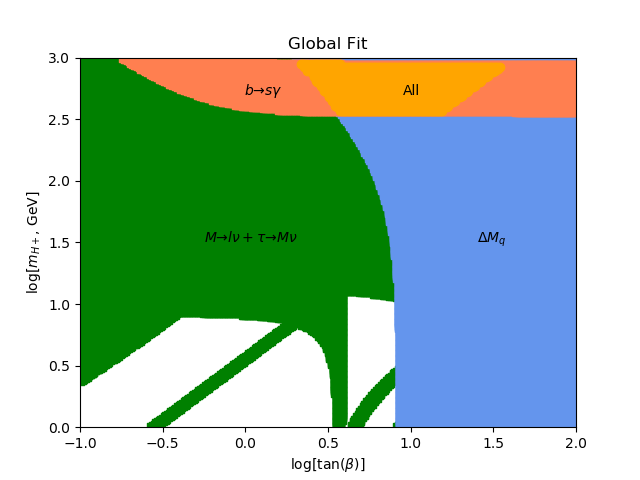
\includegraphics[scale=0.8]{../calcs/global.png}
    \caption{\label{fig:glob} Global fit, tadaaaaa}
\end{figure}

\section{Next Steps}
\begin{itemize}
    \item SM4
    \item SM4 and Higgs
    \item more Higgs
    \item Z' model and comparison to Higgs, join with Higgs?
    \item something else?
\end{itemize}

%\appendix
%\section{Some title}
%Please always give a title also for appendices.
%
%\acknowledgments
%This is the most common positions for acknowledgments. A macro is
%available to maintain the same layout and spelling of the heading.
%
%\paragraph{Note added.} This is also a good position for notes added
%after the paper has been written.

% The bibliography will probably be heavily edited during typesetting.
% We'll parse it and, using the arxiv number or the journal data, will
% query inspire, trying to verify the data (this will probalby spot
% eventual typos) and retrive the document DOI and eventual errata.
% We however suggest to always provide author, title and journal data:
% in short all the informations that clearly identify a document.

\begin{thebibliography}{99}

\bibitem{a}
O. Deschamps et al, \emph{The Two Higgs Doublet Model of Type II facing flavour physics data}, \href{https://arxiv.org/pdf/0907.5135.pdf}{arxiv:0907.5135}.

\bibitem{b}
G. Degrassi, P. Gambino, and P. Slavich, \emph{SusyBSG: a fortran code for} BR$[B\to X_s\gamma]$ \emph{in the MSSM with Minimal Flavor Violation}, \href{https://arxiv.org/pdf/0712.3265.pdf}{arxiv:0712.3265}.

\bibitem{c}
Y. Amhis et al [HFLAV], \emph{Averages of b-hadron, c-hadron, and $\tau$-lepton properties as of 2018}, \href{https://arxiv.org/pdf/1909.12524.pdf}{arxiv:1909.12524}.

\bibitem{d}
M. Tanabashi et al [Particle Data Group], Phys. Rev. D98, 030001 (2018) and 2019 update

\bibitem{e}
A. Sibidanov et al [Belle], \emph{Study of Exclusive $B\to X_ul\nu$ Decays and Extraction of $|V_{ub}|$ using Full Reconstruction Tagging at the Belle Experiment}, \href{https://arxiv.org/pdf/1306.2781.pdf}{arxiv:1306.2781}.

\bibitem{f}
A. Lenz and G. Tetlalmatzi-Xolocotzi, \emph{Model-independent bounds on new physics effects in non-leptonic tree-level decays of B-mesons}, \href{https://arxiv.org/pdf/1912.07621.pdf}{arxiv:1912.07621}.

\bibitem{g}
CKMfitter Group (J. Charles et al.), Eur. Phys. J. C41, 1-131 (2005) [hep-ph/0406184], updated results and plots available at: \href{http://ckmfitter.in2p3.fr}{http://ckmfitter.in2p3.fr}.

\bibitem{h}
A. Sakharov, \emph{Violation of CP Invariance, C asymmetry, and Baryon Asymmetry of the Universe}, Pisma Zh. Eksp. Teor. Fiz. 5 (1967) 32 [JETP Lett. 5 (1967) 24] [Sov. Phys. Usp. 34 (1991) 392] [Usp. Fiz. Nauk 161 (1991) 61].

\bibitem{i}
L. Di Luzio, M. Kirk, A. Lenz, T. Rauh, \emph{$\Delta M_s$ theory precision confronts flavour anomalies}, \href{https://arxiv.org/pdf/1909.11087.pdf}{arxiv:1909.11087}.

\bibitem{j}
S. Aoki et al [FLAG], \emph{FLAG Review 2019}, \href{https://arxiv.org/pdf/1902.08191.pdf}{arxiv:1902.08191}.

\bibitem{k}
A. Lenz, private correspondence.

\bibitem{l} %CKM ref
J.F. Donoghue, E. Golowich, and B.R. Holstein, \emph{Dynamics of the Standard Model} (Cambridge University Press, 2014).

\bibitem{m} %covar deriv
G. Kane, \emph{Modern Elementary Particle Physics} (Addison-Wesley, 1987).

\bibitem{n} %gauge transforms
D. Bailin and A. Love, \emph{Introduction to Gauge Field Theory} (Institute of Physics, 1993).

\bibitem{o} %Higgs
M.D. Schwartz, \emph{Quantum Field Theory and the Standard Model} (Cambridge University Press, 2018).



% Please avoid comments such as "For a review'', "For some examples",
% "and references therein" or move them in the text. In general,
% please leave only references in the bibliography and move all
% accessory text in footnotes.

% Also, please have only one work for each \bibitem.


\end{thebibliography}
\end{document}
